\documentclass[9pt,twocolumn,twoside]{../../styles/osajnl}
\usepackage{fancyvrb}
\journal{i524} 

\title{Analysis of Airline delays data using Spark and HDFS}

\author[1,*]{Bhavesh Reddy Merugureddy}
\author[1,**]{Niteesh Kumar Akurati}


\affil[1]{School of Informatics and Computing, Bloomington, IN 47408, U.S.A.}

\affil[*]{Corresponding authors:bmerugur@iu.edu}
\affil[**]{Corresponding authors: akuratin@iu.edu}


\dates{project-P014, \today}

\ociscodes{Ansible, Spark, Cloudmesh Client, Hadoop, YARN}

% replace this with your url in github/gitlab
\doi{\url{https://github.com/cloudmesh/classes/blob/master/project/S17-IR-P014/report/report.pdf}}


\begin{abstract}

Airline delays data is analyzed by developing an automated process for
deploying Hadoop and Spark on Chameleon and Jetstream cloud computing
environments. The data set used is publicly available and analyzed for
obtaining various results like average delay of an airline and an
airport. The automation process is carried out using Ansible scripts
and a cloud manager called Cloudmesh Client is used to interact with
the clouds. Spark is used as the cluster computing framework and
Hadoop Distributed File System is used as the distributed storage
system for the data sets. Benchmarking is done after the analysis to
determine the efficiency and performance of the system.
\newline
\end{abstract}

\setboolean{displaycopyright}{true}

\begin{document}

\maketitle



\section{Introduction}

Analysis of airline delays data by deployment of Hadoop and Spark on
Chameleon and Jetstream clouds is the main focus of the project. A
data set having the airlines information such as flight arrival time,
departure time and average delays is considered. This data set is
available to everyone. Cloudmesh Client is used as the cloud manager
which provides command line to access multiple clouds. It is used to
create a Hadoop cluster with Spark as an add-on. The cluster is then
deployed on Chameleon and Jetstream clouds by using the Cloudmesh
Client. Ansible scripts are written and the Cloudmesh Client interacts
with these scripts to automate the deployment.

Ansible scripts are written for extracting data sets from the
published zip file and deploying them on the clouds. Hadoop
Distributed File System is used to store the extracted data sets. A
program is written in Spark to perform the data analysis. Spark runs
on the Hadoop cluster and accesses the HDFS for retrieving the data
sets. There are several results that are obtained from this
analysis. Top ten airports that have delays are identified, average
delay per an airline and per an airport is determined and top ten
airlines with comparatively more delays are identified.

The program is deployed by using an Ansible script. Bar graphs are
drawn for the analysis performed. Along with the deployment and
analysis, benchmarking is done to evaluate the performance of the
program on each node of a cluster and on different clouds. The
efficiency of the program is determined by varying the sizes of the
data set and comparing the results.

\section{Infrastructure} 

Infrastructure for the project includes Cloudmesh Client, Chameleon
and Jetstream clouds. Cloudmesh Client is used to access multiple
clouds from a single command line. Chameleon and Jetstream provide
cloud computing environments for the system.

Cloudmesh Client is a toolkit that provides a standardized interface
for accessing various workstations, clusters and heterogeneous
clouds. It acts as a manager that allows users to manage the available
set of resources. Cloudmesh Client plays an essential role in the
deployment process by handling the interactions between users and
virtual machines being used in the clouds
\cite{cloudmeshClientdoc}.

Cloudmesh Client provides several services which make it easy for the
users to manage the virtual machines in the clouds. The “vm boot”
command in Cloudmesh Client is a single instruction for creating
virtual machines. Security rules can be uploaded to the clouds by
using “secgroup” command from Cloudmesh. Key management in the clouds
is simplified Cloudmesh’s key add and upload commands. Deletion of the
virtual machines created can be easily carried out by specific
commands defined in Cloudmesh.

Cloudmesh Client makes it easy for the users to switch virtual
machines from one cloud to other by specifying the name of the
cloud. Cloudmesh provides a command shell that allows users to develop
and run scripts and each command can be called by the user from the
command line. Cloudmesh Client essentially provides virtual machine
management through a convenient programmable interface.



\subsection{Chameleon Cloud}

Chameloen is a project aimed at providing large-scale open research
platform for cloud design and services. The project receives funding
from the National Science Foundation (NSF). Chameleon provides a wide
range of services like developing platforms-as-a-service, optimizing
virtualization technologies and infrastructure-as-a-service components
\cite{chameleonDoc}. Chameleon allows full user configurability of the
software stack, ranging from provisioning of bare metal to the
delivery of high functioning cloud environments, by supporting a
graduated configuration system.

The Chameleon testbed is hosted at the University of Chicago and the
Texas Advanced Computing Center. It consists of 5PB of total disk
space with 650 multi-core cloud nodes. A portion of the testbed is
dedicated for supporting experiments with large disk, high memory and
co-processor units. Chameleon facilitates integration of clouds and
networks enhancing their capabilities.


\subsection{Jetstream}

Jetstream is a cloud computing environment that can be used by
researchers as a configurable infrastructure. They are provided with
interactive computing and data analysis resources
\cite{jetIu}. Jetstream allows researchers to create their own private
computing system with customizable virtual machines. Jetstream’s
operational software environment is based on OpenStack and has a
web-based user interface. It provides a library of virtual machines
for performing specific analysis tasks. It can be used for tailoring
workflows for both small scale and larger scale environments. It can
also be used as the backend to science gateways to supply research
jobs to HTC or other HPC resources.

Table 1 shows the specifications used from both Jetstream and
Chameleon cloud environments.

\begin{table}[htbp]
\centering
\caption{\bf Hardware Specifications of Chameleon and Jetstream}

 \begin{tabular} {| c | c | c |}
\hline
  & Chameleon  & Jetstream \\ [0.5ex] 
 \hline

    
CPU     & Xeon X5550 & Haswell E-2680  \\
 \hline
cores &        1008   &  7680 \\
 \hline
speed     &               2.3GHz & 2.5GHz\\
 \hline
RAM   &               5376GB  &  40TBr\\
 \hline
storage     &                   1.5PB  & 2 TB\\ [1ex] 
 \hline

\end{tabular}
  \label{tab:cloud-comparison}
\end{table}

\section{Software Stack} 

Following are the deployment and analysis tools used in the project.

\subsection{Ansible}

Ansible is an open-source software that facilitates automation of
configuration management and application deployment. Ansible consists
of controlling machines and nodes. Controlling machine starts the
orchestration and manages the nodes over SSH
\cite{ansibleWiki}. Resources are not consumed by Ansible when the
nodes are not being managed. This is due to the fact that there are no
daemons that run for Ansible in the background. This makes Ansible a
software with an agent-less architecture. This architecture prevents
the nodes from polling the controlling machine thereby reducing the
overhead on the network as shown in figure 1.

\begin{figure}[ht]
  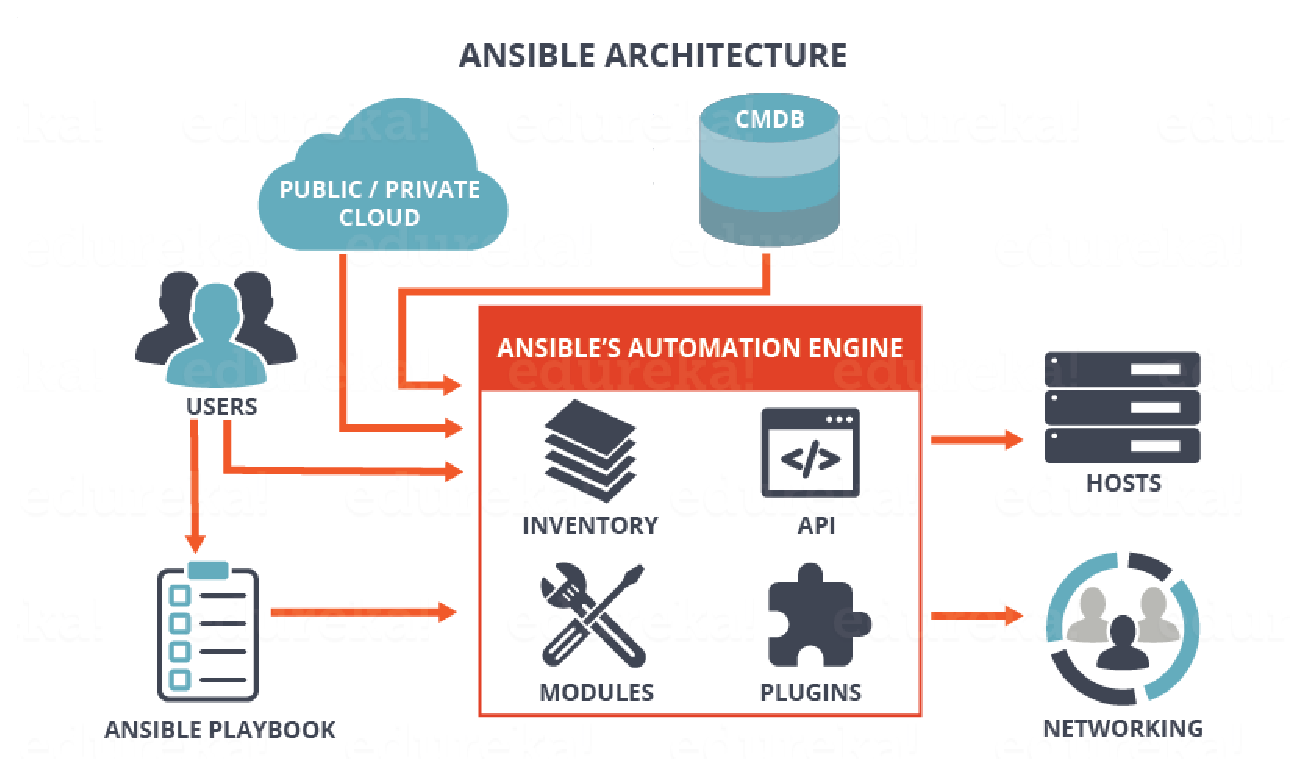
\includegraphics[scale=0.4]{images/ansible_architecture.eps}
  \caption{Ansible Architecture} \cite{ansibleArch}
\end{figure}

Modules, Inventory, Playbooks and Ansible Tower are the components of
the Ansible architecture. In Ansible, a module is work unit written in
a scripting language. It is idempotent and standalone. Inventory is a
configuration file that lists the nodes that are accessible by
Ansible. It allows the users to add a set of nodes to a group. Nodes
are generally represented by IP addresses or hostnames.

Playbooks are YAML format files which consist of configurations and
express deployment in Ansible. A group of hosts are mapped to a set of
roles through Playbook. Ansible Tower is a web-based console which
makes Ansible a center for automating tasks. Ansible is consistent and
minimal in nature. Ansible does not deploy agents to nodes which makes
it very secure.

\subsection{Apache Spark}

Apache Spark is an open source framework that provides
cluster-computing capabilities. Spark allows its users to program
different clusters by providing an interface \cite{sparkWiki}. It
facilitates fault-tolerance and data parallelism. Spark makes use of a
data structure called as resilient distributed dataset (RDD) which is
distributed over different virtual machines in a cluster.

RDDs are immutable which means that they cannot be changed once they
have been created. They provide mechanisms for exploratory data
analysis and iterative algorithms for processing dataset
iteratively. Spark interfaces with systems like Cassandra, Hadoop
Distributed File System (HDFS) and Amazon S3 for distributed storage
and interacts with Hadoop YARN for cluster management.

Task scheduling, dispatching and some fundamental I/O functionalities
are achieved in Spark through the Spark Core. It is an application
programming interface which reflects functional programming. Functions
similar to map and reduce are provided by the interface which produces
new RDDs as output by taking in the required RDDs. RDDs make use of
different types of Java, Scala or Python objects. The operations of
RDDs are fault-tolerant and lazy. Structured and semi-structured data
is supported in Spark through Spark SQL that processes a new data
model called DataFrames. Spark SQL provides ODBC/JDBC server and
command-line interfaces.

RDD transformations are performed on the data by the Spark Streaming
component. It takes in data and performs streaming analytics. Spark
MLlib is a machine learning framework that simplifies machine learning
pipelines in Spark \cite{sparkWiki}. MLlib is provided with several
statistical and machine learning algorithms. This reduces the overhead
of performing classification and regression, correlations, linear
regression, support vector machines and k-means clustering method. A
simple spark architecture can be observed in figure 2. Apache Spark
consists of a graph processing component known as GraphX. It depends
on RDDs and generally used for graphs that are immutable.

\begin{figure}[ht]
  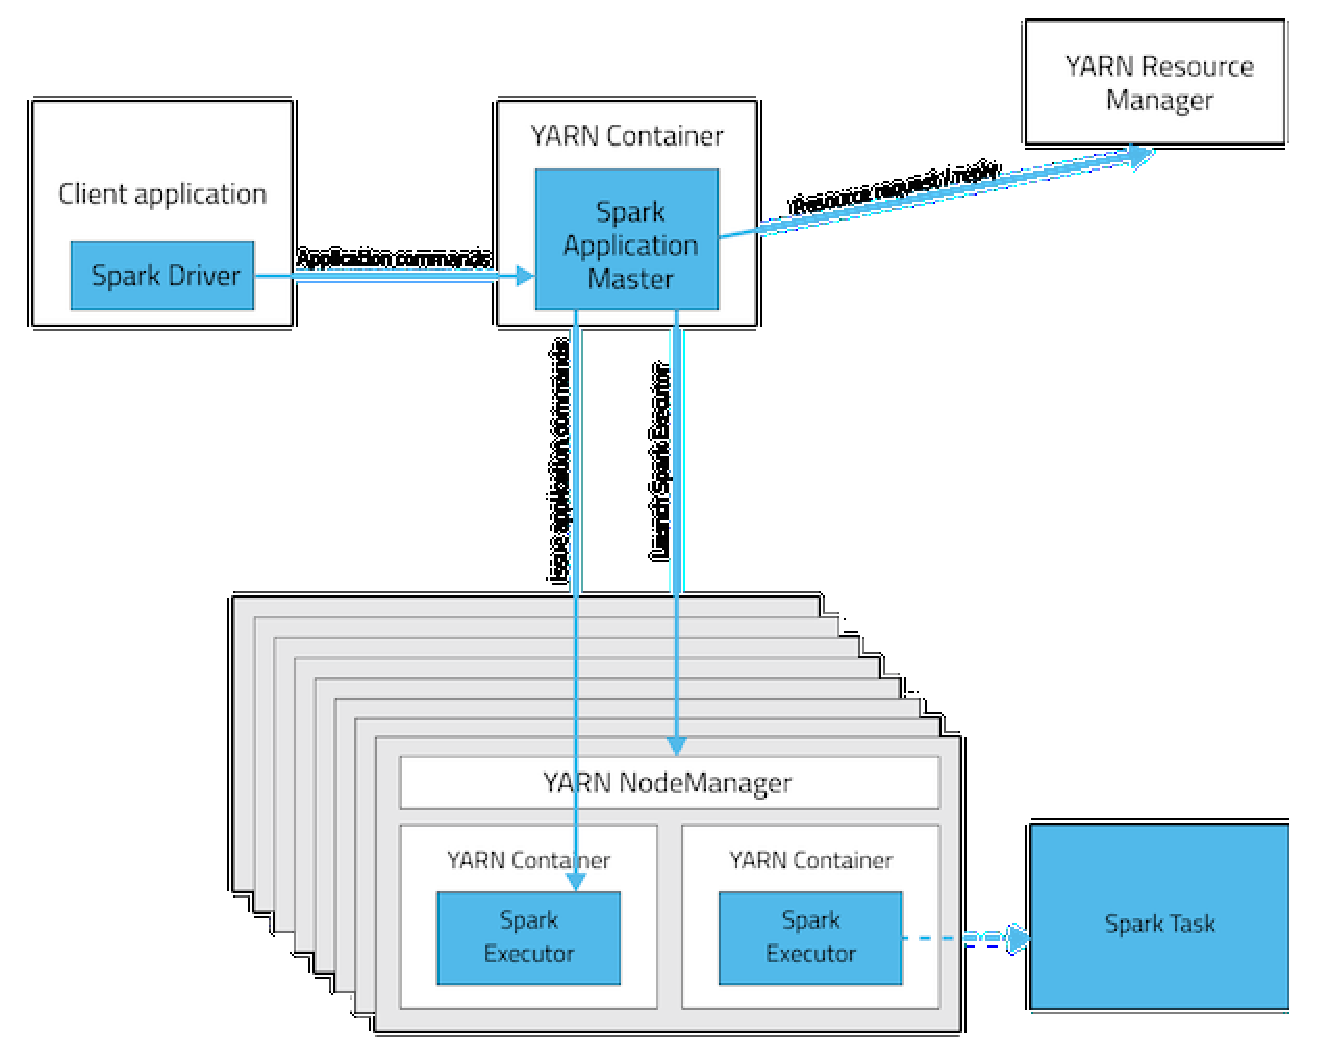
\includegraphics[scale=0.35]{images/sparkYarn.eps}
  \caption{Spark with Yarn Architecture} \cite{sparkwithYarn}
\end{figure}

Generally, map and reduce functions use variables which are defined
outside the functions in Spark driver. New copies of each variable are
provided to the tasks running on the cluster but the driver is not
provided with the updates of these copies \cite{accumulatorSpark}. To
solve the problem, Spark makes use of shared variables called
accumulators. An accumulator can be considered as a container used for
aggregating data across different tasks running on multiple executors.

Accumulators are designed for distributed sums and counters and can be
effectively used for distributed computations
\cite{accumulatorGit}. They act as read-only variables for the
executors and can only be read by the driver programs. Accumulators
are not thread-safe but they are serializable. They can be safely sent
over the wire for execution after being referenced in the code in
executors. Accumulators even help in the debugging process by counting
the events.


\subsection{Hadoop Distributed File Systen}

The Hadoop Distributed File System (HDFS) is a distributed file
storage system that provides reliable and scalable data storage. It is
a fault-tolerant storage system. It spans large clusters of commodity
servers \cite{hdfsHorton}. It supports thousands of servers and a
billion files. HDFS distributes storage and computation across many
servers making the combined storage resource grow with demand and
remain economical at every amount of storage.

HDFS allows the users to connect the nodes across several clusters in
which the data is distributed. It provides high throughput access to
large datasets \cite{hdfsIbm}. The data files can be accessed by the
users in a streaming manner as the data files are stored as a
continuous file system. MapReduce programming model is employed when
applications are executed. HDFS has a write-once-read-many model which
simplifies data coherency and lightens the requirements of concurrency
control. It allows only one writer to write data at a given point of
time. It appends bytes to the end of a stream and stores the streams
in the order they were written.

HDFS provides portability across heterogeneous operating systems and
ensures efficiency by processing the distributed data in parallel. It
automatically redeploys processing logic in the failure situations by
maintaining multiple copies of data. Rather than processing data close
to logic, HDFS processes logic closer to data. It is accessible in
different ways. 

A web browser can be used to browse files in HDFS. It consists of a
single node called name node and several data nodes that store data as
blocks within the files. The name node is responsible for regulating
client access to files and managing the namespace of the file
system. This includes opening, closing and renaming files and
directories. Name node monitors the data nodes in creating, deleting
and replicating data blocks by mapping them to the data nodes. Each
data node contains an open server socket through which remaining data
nodes read or write data.

To be fault-tolerant, HDFS replicates file blocks according to the
number that an application specifies. It optimizes replica placement
by using an intelligent replica placement model which in turn, ensures
reliability and efficiency. HDFS supports large files by placing each
file block on a different data node. To overcome failures, it makes
use of heartbeat messages for detecting connectivity between data
nodes and the name node. Data nodes are required to send heartbeat
messages to the name node periodically and the failure is detected
when name node stops receiving the messages. In this situation, the
data node is marked as dead and removed from the system. When the data
node count reaches a limit value, replication is done by the name
node. Figure 3 shows the architecture of HDFS.

\begin{figure}[ht]
  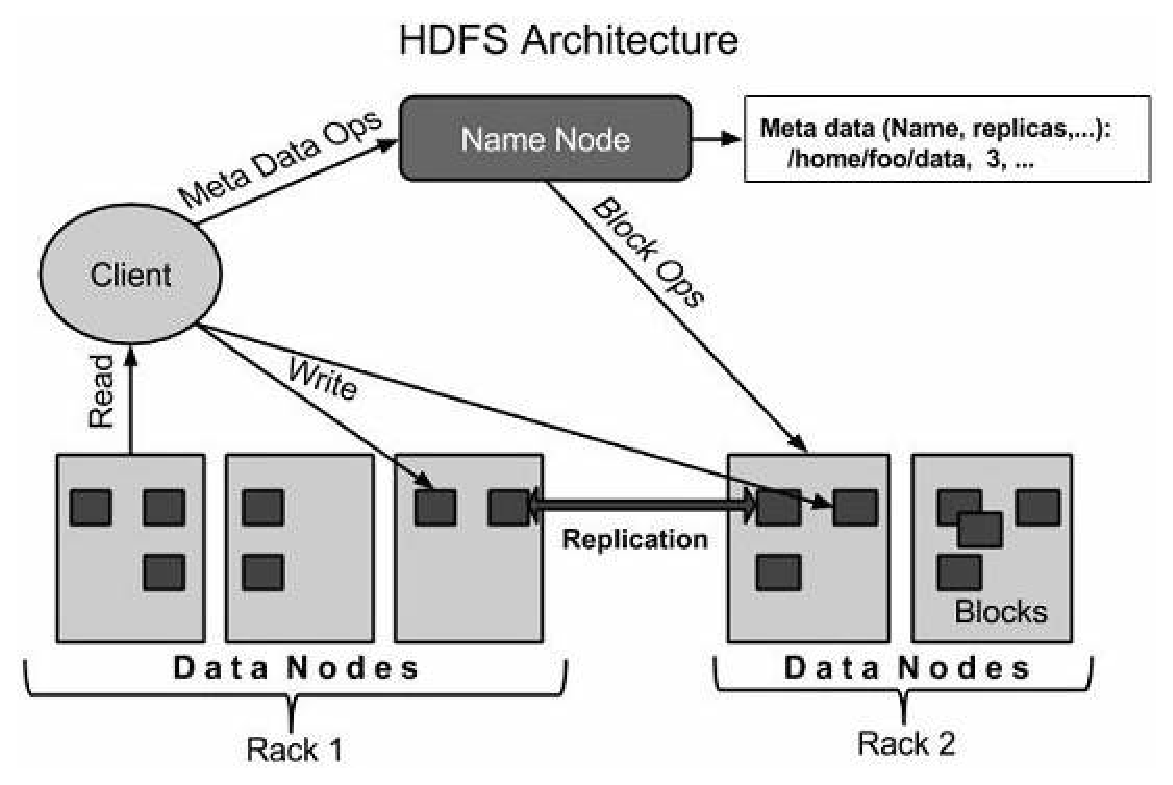
\includegraphics[scale=0.45]{images/hdfs_architecture.eps}
  \caption{HDFS Architecture} \cite{hdfsArch}
\end{figure}

HDFS supports data block rebalancing to avoid the used space for data
nodes from being underutilized. If the free space on a data node is
too low, it automatically moves blocks from one data node to
other. Rebalancing is also done when new nodes are added to the
cluster. It ensures integrity of data stored in HDFS. The file system
performs checksum validation on the files by storing computed
checksums in separate files in the namespace of actual data
\cite{hdfsIbm}. All other HDFS functionalities are similar to that of
other distributed file systems.



\subsection{YARN}

Yet Another Resource Negotiator (YARN) is a technology used for
cluster management. Hadoop supports a broad range of applications
through YARN as it decouples MapReduce’s scheduling mechanism and
resource management from the data processing component
\cite{yarnDef}. YARN consists of a node manager and a central resource
manager. Node manager monitors the operations of cluster nodes while
the resource manager manages the Hadoop system resources which are
used by the applications. YARN separates HDFS from MapReduce which
improves the efficiency of the Hadoop environment in processing
different operations.

The resource manager is responsible for governing a cluster by
assigning applications to the underlying resources. Resources like
bandwidth and memory are orchestrated by the resource manager to the
underlying node managers \cite{yarnIbm}. Applications that run within
YARN are managed by the ApplicationMaster. YARN allocates resources
through ApplicationMasters and monitors the underlying applications
through node managers. ApplicationMasters are responsible for
execution of containers and negotiation of resources from the resource
manager. They are assumed as buggy as they are user code and a
security issue.

The node manager manages the nodes within a cluster by providing
per-node services within that cluster. YARN uses the data nodes and
name nodes from HDFS layer. Data node is used for replicated storage
services across a cluster while the name node is used for metadata
services. Execution of YARN is initiated by a client application that
sends a request. ApplicationMaster is then triggered by resource
manager to represent the application.

In the cluster, the ApplicationMaster negotiates containers for the
application at each node by making use of a resource-request
protocol. After the completion of the application, it unregisters the
containers from the resource manager. YARN improves the ability to
scale Hadoop clusters to large confiurations by reducing the overhead
on resource manager and making the ApplicationMaster responsible for
the management of job execution. Moreover, it allows a parallel
execution of different programming models like machine learning and
graph processing.

YARN allows users to create distributed applications which are more
complex than the ones developed by the traditional MapReduce
paradigm. It provides a scope for customized development by exposing
the underlying framework \cite{yarnIbm}. This makes it more robust and
it does not need to be segregated from other distributed frameworks
that reside on the cluster. YARN frees up resource overhead that has
been dedicated to the distributed frameworks which simplifies the
complexity of the overall system.

As YARN provides customized development, it becomes more difficult to
build YARN applications. This is due to the development of
ApplicationMaster which is required after launching resource manager
on a client request. YARN initially allocates a certain number of
resources within a cluster. It processes the application and provides
touchpoints to monitor the progress of the application. After this
process, it releases resources and performs a cleanup when the finds
the status of the application as complete. YARN provides many services
which are beyond the scope of traditional MapReduce. 


\section{Dataset}

Airlines delay data set is used as the data for analysis. It is
analyzed using Pyspark. It is published by the United States
department of transportation as the flight related information. This
data is free for anyone to use and analyze. Here, we get flight
arrival and departure times and delays for all flights taking off in a
certain period.

Data is obtained by mentioning a year or a period of time within which
the flight information is required. Three files containing this
information namely airlines.csv, airports.csv and flights.csv are
available in the form of a zip file. The flights.csv file contains the
following fields: Flight ID, airline, airport, departure, arrival and
delay. Airlines.csv has airline ID and airline name. The airports.csv
file consists of airport ID and airport name. These files are placed
in the local file system or in HDFS. The spark program reads the files
from either location. If the files are placed in HDFS, “hdfs://” is
to be given as a prefix to the file path.


\section{Deployment} 


The deployment process is driven by Ansible playbooks and Cloudmesh
Client commands and scripts. The process is initiated on user’s local
Ubuntu instance. The commands are executed in local machine as well as
virtual machines on the cloud.

\begin{itemize}

\item Cloudmesh Client is used to access multiple clouds from the
  command line. This makes it easier to switch to another cloud in
  case of a failure. 
  
  
\item After the Cloudmesh Client installation, ssh key is to be added
  to the Cloudmesh database and uploaded to all the active clouds.

\item The configuration file of the Cloudmesh Client is to be modified
  by making Chameleon and Jetstream as active clouds.

\item Security rules are then added to the user’s security profile
  after which security group is uploaded to communicate with the
  virtual machines.

\item A virtual cluster is to be created on the cloud by specifying the number of nodes. 
\end{itemize}

Cloudmesh provides one line command for doing so. In order to make use
of the nodes, floating IPs need to be assigned to the created
nodes. Cluster creation fails when the cloud runs out of floating
IPs. Floating IP is required for the communication between the servers
and ssh from the client to the cloud. A Hadoop cluster is defined on
top of the cluster we defined. Table 2 shows the resources on the
cloud that have been used.


\begin{table}[htbp]
\centering
\caption{\bf Resources on clouds}

 \begin{tabular}{|c | c | c|} 
 \hline
&  Chameleon & Jetstream \\ [0.5ex] 
 \hline\hline
    
Flavor &	m1.medium &	m1.medium \\
 \hline
OS&	Ubuntu 14.04 &	Ubuntu 14.04 \\ 
 \hline
secgroup &	default &	default \\ 
 \hline
Nodes &	3 &	3 \\ [1ex] 
 \hline

\end{tabular}
  \label{tab:fault-tolerance}
\end{table}

\begin{itemize}
  
\item Similar to the cluster previously defined, multiple
  specifications can be defined for the Hadoop cluster and one
  specification has to be activated.

\item After this, Hadoop cluster can be deployed by synchronizing the
  Big Data stack.

\item To use Spark as an add-on in the Hadoop cluster, Spark is to be
  passed as an argument while defining the Hadoop cluster.

\item The details of the specification of the Hadoop cluster can be
  viewed by using the “cm hadoop avail” command.

\item The Spark cluster can then be deployed by using “cm hadoop sync”
  and “cm hadoop deploy” commands.

\item The process of uploading the data set to HDFS and running the
  Spark program on the uploaded data set is automated through an
  Ansible script.

\item Installing the analysis code into the repository is also automated.
\end{itemize}

\section{Analysis}

Airlines dataset publicly available from US Government website is used
for performing analysis and finding out various insights. The dataset
is downloaded by identifying the goals to be accomplished. The dataset
consists of three files, they are flights.csv, airlines.csv,
airports.csv.  The flights.csv has key informtion like the departure,
delay of various airlines and airports. The airlines.csv and
airports.csv files contains the code for an airline and airport
respectively and their corresponding names.  The airline and airport
files can be used as lookup files. The flight data is the key for the analysis.

Initially, the flight data is parsed to create a flight tuple with all
the fields in the flight class to be members of the named tuple, just
like class and its objects. The following functions are implemented
they are parse, split and notHeader. Parse is used to parse each
indiviual row in the flights.csv and convert it into a named
tuple. The split function is used to split each column value in a row
based on comma since the dataset is comma seperated values. After
loading the SparkContext, the airlines data is parsed to eliminate the
header and split it accordingly.

Similarly, the airports data is parsed.  The flights data is parsed
such that each individual row is converted into a named tuple.  By
using this parsed data, output is obtained by performing various
transformations and actions.

The process is to transform the flights RDD by applying filters and
map functions for getting the delay based on two instances i.e,
airports and airlines. Then ReduceByKey and CombineByKey actions are
performed by aggregating and computing the average delay in case of
each airport and sorting functions are applied to sort the output in
descending order and based on that, the top ten airports to avoid are
obtained given the average delay per airport. Since the codes of
various airlines and airports are the only ones available, lookup
operations are performed by using countAsMap() operation with airports
and airlines dataset and by using broadcast, the lookup information is
passed on to all workers and executors within them.

The top ten airlines to avoid are found by computing the total minutes
of delay per airline over a period of time. Figure 4 shows the top
ten airlines obtained by the analysis. The analysis can be further
improvised by using various Machine Learning techniques which helps in
predicting the delays over a period of time ahead and provides various
insights which are helpful in making better decisions in choosing
airlines and airports to commute.


\begin{figure}[ht]
  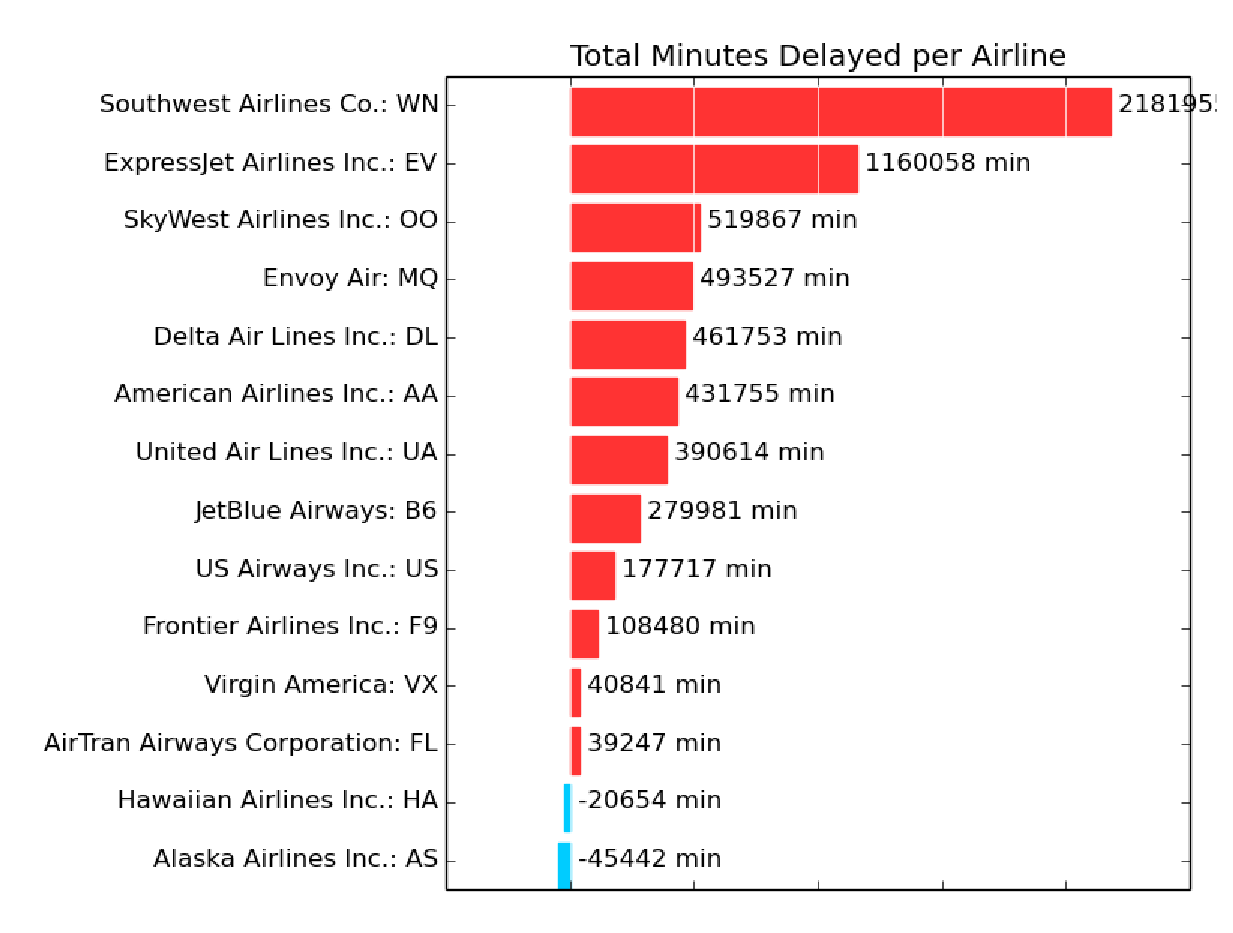
\includegraphics[scale=0.40]{images/airlinesAnalysis.eps}
  \caption{Top ten airlines to avoid}
\end{figure}

\section{Benchmarking}

Benchmarking is carried out after the deployment and data analysis. It
is done to evaluate the efficiency and performance of the system. As a
part of benchmarking, the flight and airline data analysis performed
is evaluated by running the code on Jetstream and Chameleon cloud
computing environments.

The data is transferred to Hadoop Distributed file system and analysis
is done by using Spark with YARN. To evaluate the efficiency of the
analyis, the dataset has been used in varying sizes. Datasets with
increasing size in rows have been considered for this purpose. As it
is known that the transformations in Spark are lazy, the results are
not evaluated right away. This makes it even more efficient.

Python's time module is used for obtaining the current time. Time for
running the analysis is found out by determining timestamps both
before and after running the code, named beforeTime and afterTime
respectively. The required time is determined by subtracting
beforeTime from afterTime. Due to Spark's lazy evaluation, the time
module used is wrapped around the Spark actions. Figure 5 shows the
time, in seconds, taken by the analysis in Jetstream cloud computing
environment with different dataset sizes.

\begin{figure}[ht]
  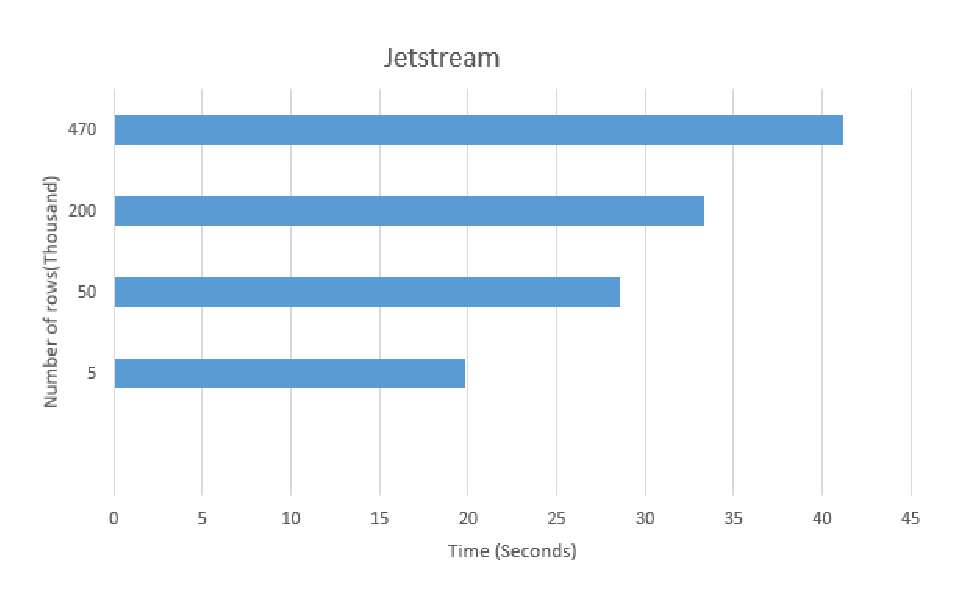
\includegraphics[scale=0.50]{images/jsBench.eps}
  \caption{Performance on Jetstream}
\end{figure}

Figure 6 shows the performance of the analysis on Chameleon cloud
environment.

\begin{figure}[ht]
  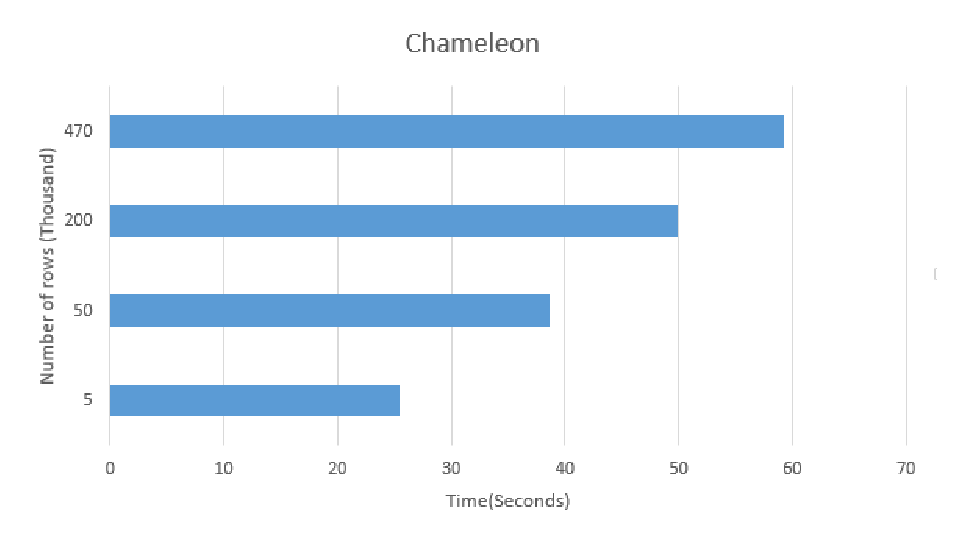
\includegraphics[scale=0.50]{images/ccBench.eps}
  \caption{Performance on Chameleon}
\end{figure}

As the analyis code, data and packages are installed on the clusters
through Ansible playbook, the time taken for the automation on
Chameleon and Jetstream clouds is determined and the values obtained
on each cloud are compared. The comparison is shown in figure 7.

\begin{figure}[ht]
  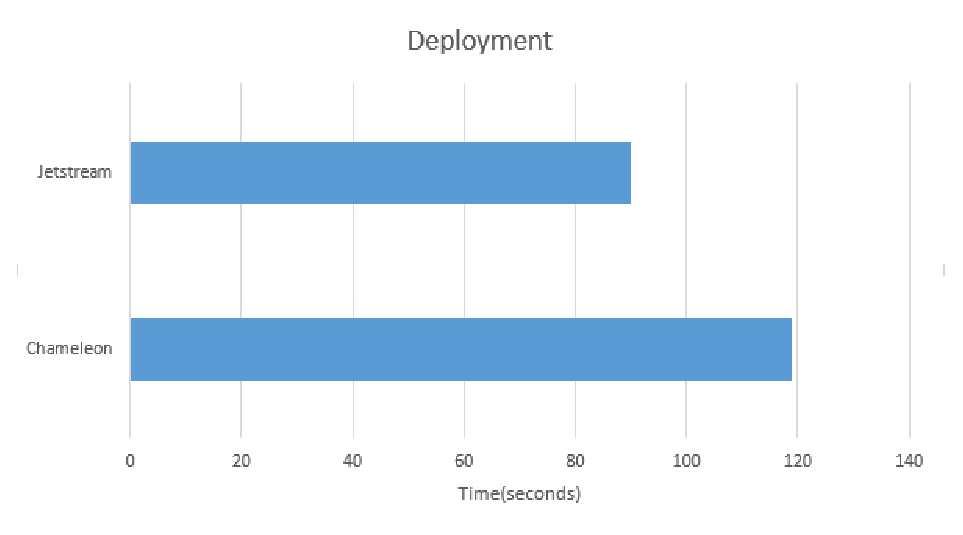
\includegraphics[scale=0.50]{images/CcVsJs.eps}
  \caption{Deployment in Chameleon and Jetstream}
\end{figure}

\section{Timeline}

Week by week timeline for project completion is specified in this section.

\begin{enumerate}

\item {March 6 - March 12, 2017: } Created virtual machines on Chameleon
  cloud using Cloudmesh.
  
\item {March 13 - March 19, 2017: } Deployed Hadoop cluster to Chameleon
  cloud using Cloudmesh.

\item {March 20 - March 26, 2017: } Acquired data for performing
  analysis and submitted the project proposal.

\item {March 27 - April 02, 2017: } Created virtual machines on
  Jetstream cloud using Cloudmesh and deployed Hadoop cluster to the
  cloud using Cloudmesh.

\item {April 03 - April 09, 2017: } Perfomed analysis on the data using
  Apache Spark on top of Hadoop stack.
  
\item {April 10 - April 16, 2017: } Developed Ansible playbook to deploy
  Hadoop and Spark to the cloud machines. 

\item {April 17 - April 23, 2017: } Completed project report and developed
  benchmarks for the project.

\end{enumerate}


\section{work breakdown} 

Below is the work distribution for the implementation, testing and documentation of the project.

\begin{itemize}
\item Bhavesh Reddy Merugureddy
    \begin{itemize}
    \item Creating and deploying clusters on Jetstream.
    \item Acquiring the data and performing analysis on flight data.
    \item Writing transformations and actions required for the
      analysis using Spark.
    \item Setting up and testing the end to end flow on Jetstream cloud.
    \item Performing benchmarking for the analysis on Jetstream by
      varying the data set size.
    \item Writing related sections in this report.
    \end{itemize}

\item Niteesh Kumar Akurati
    \begin{itemize}
    \item Creating and deploying clusters on Chameleon.
    \item Collecting airport data and performing analysis. 
    \item Implementation of Ansible scripts for deployment of code,
      data and the required packages.
    \item Setting up and testing the end to end flow on Chameleon cloud.
    \item Performing benchmarking for the analysis on Chameleon by
      varying the data set size.
    \item Writing related sections in this report.
    \end{itemize}
\end{itemize}

\section{Conclusion} 

Airline delays data has been analyzed by the deployment of Hadoop and
Spark on Chameleon and Jetstream cloud computing environments. A
publicly available data set containing flight and airline related data
is taken for analysis. Cloudmesh Client is used as the cloud manager
to access multiple clouds and deploy a Hadoop cluster on Chameleon and
Jetstream clouds. Ansible scripts are written for extracting data sets
from the published zip file and deploying them on the clouds. Hadoop
Distributed File System is used to store the extracted data sets. A
program is written in Spark to perform the data analysis which is
deployed by using an Ansible script. Bar graphs are drawn for the
analysis performed. Apart from the deployment and analysis,
benchmarking is done to evaluate the performance of the program on
each node of a cluster and on different clouds. The efficiency of the
program is determined by varying the sizes of the data set and
comparing the results.

\section{Acknowledgements}

This project is undertaken as part of the I524: Big Data and Open
Source Software Projects coursework at Indiana University. We would
like to thank our Prof. Gregor von Laszewski, Prof. Gregory Fox and
the Associate Instructors for their help and support.

\bibliography{references}

\end{document}
